\documentclass[aspectratio=169]{beamer}
\usepackage[utf8]{inputenc} % codificacao de caracteres
\usepackage[T1]{fontenc}    % codificacao de fontes
\usepackage[english]{babel}  % idioma
\usepackage{graphics,amssymb,amsfonts,amsmath}
\usepackage{tikz}
\usepackage{enumerate,hyperref}
\usepackage{palatino}	% Fonte sem serifa
\usepackage{ragged2e}	% Paragrafo justificado
%\usepackage{minted}	% Highlight para codigos de programacao
\usepackage{booktabs} % tabelas
\usepackage{multicol}
\usepackage{multirow}

%\usepackage[table]{xcolor}


% Veja mais temas e cores em http://www.hartwork.org/beamer-theme-matrix/
\usetheme{Montpellier}         % tema
\usecolortheme{orchid}      % cores
\usefonttheme[onlymath]{serif} % fonte modo matematico
% Colocando numero de paginas no slide
\setbeamertemplate{footline}[frame number]



\DeclareGraphicsExtensions{.pdf,.JPG,.png} % compilamos apenas com pdflatex
%\graphicspath{{./figuras/}} % caminho onde as figuras estarao disponiveis


\graphicspath{{figuras/}}

% ---------------------------------------------------------------------------- %
% T�tulo                                                                       %
% ---------------------------------------------------------------------------- %

\title[\sc{Teoria de Circuitos Eletrônicos 1}]{\LARGE Aula 6: The Operational Amplifier}
\author[Prof. Marcelino Andrade]{Prof. Marcelino Andrade}
\institute{Faculdade UnB Gama} % opcional
\date{\today}

\begin{document}
\justifying % Paragrafo justificado
\pagebreak

\begin{frame}
  \titlepage
\end{frame}


% ----------------- NOVO SLIDE --------------------------------
\begin{frame}{Contents\newline}

\tableofcontents
%\begin{center}	
     		Introduction to Electric Circuits by James A. Svoboda, Richard C. Dorf, 9th Edition 
     		Fundamentals of Electric Circuits by Alexander and Sadiku, 4th Edition	
%\end{center}	
\end{frame}

% ----------------- NOVA SECÇÂO -----------------------------
\section{Introduction (6.1)}
% ----------------- NOVO SLIDE --------------------------------
\begin{frame}[fragile]
	\frametitle{Introduction}
		\begin{tabular}{cc}
			\begin{columns}
				\begin{column}{1\textwidth}  %%<--- here
					This chapter introduces another circuit element, the operational amplifier, or op amp. In particular, we will see that:	\newline
		
					\begin{itemize}
						\item[$\clubsuit$]{The simplest model of the operational amplifier is the ideal operational amplifier;}
						\item[$\clubsuit$]{Circuits that contain ideal operational amplifiers are analyzed by writing and solving node equations;}	
						\item[$\clubsuit$]{Operational amplifiers can be used to build circuits that perform mathematical operations.}		
					\end{itemize}
					
				\end{column}
			\end{columns}
		
	\end{tabular}
\end{frame}

% ----------------- NOVA SECÇÂO -----------------------------
\section{The Operational Amplifier 6.2}
% ----------------- NOVO SLIDE --------------------------------
\begin{frame}[fragile]
\frametitle{The Operational Amplifier}
\begin{tabular}{r}
	\begin{columns}	\column{1\textwidth}
	The operational amplifier is an electronic circuit element designed to be used with other circuit elements to perform a specified signal-processing operation.

	\end{columns} \\
	\begin{columns}
		\begin{column}{.22\textwidth}  %%<--- here
			\begin{center}
			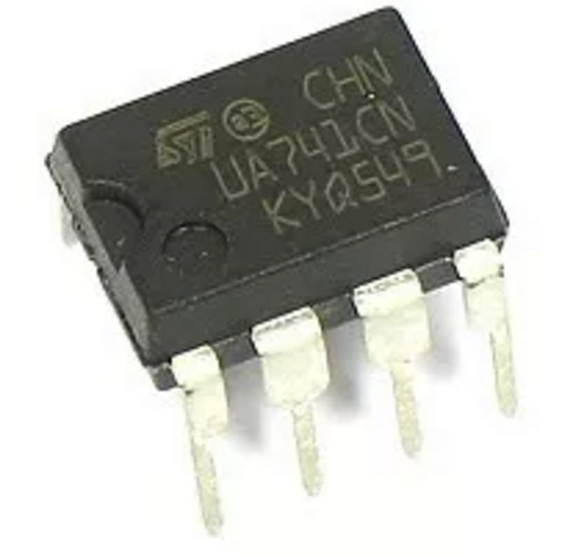
\includegraphics[height=2.5cm]{figure34.png}
			\end{center}			

		\end{column}
		\begin{column}{.24\textwidth}  %%<--- here
		\begin{center}
			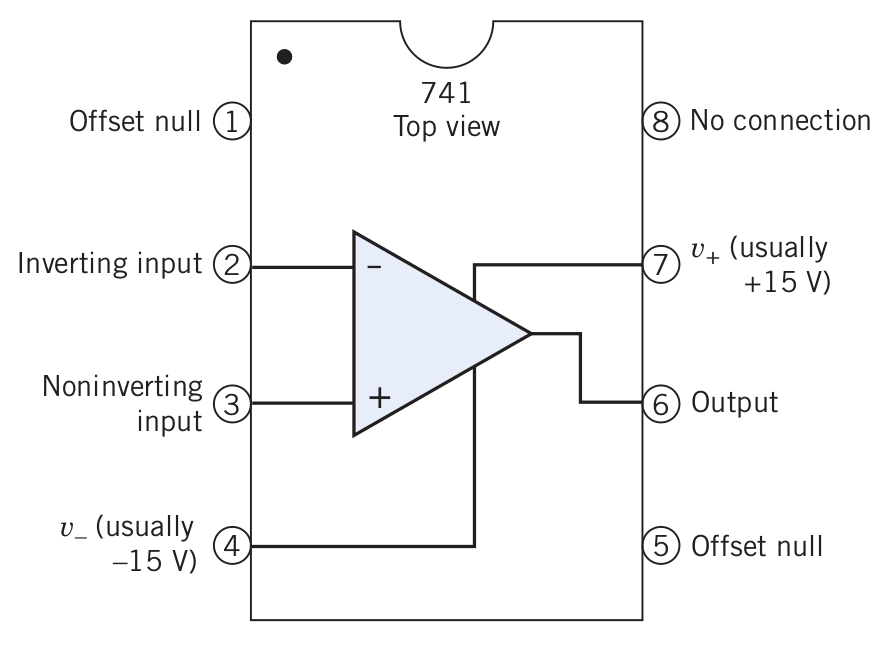
\includegraphics[height=2.5cm]{figura02.png}
			\end{center}	
		\end{column}
		\begin{column}{.24\textwidth}  %%<--- here
		\begin{center}
			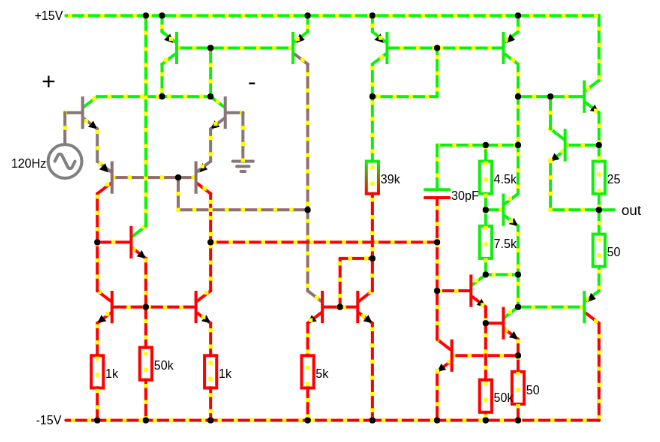
\includegraphics[height=2.5cm]{figura32.png}
			\end{center}	
		\end{column}	
		\begin{column}{.32\textwidth}  %%<--- here
		\begin{center}
			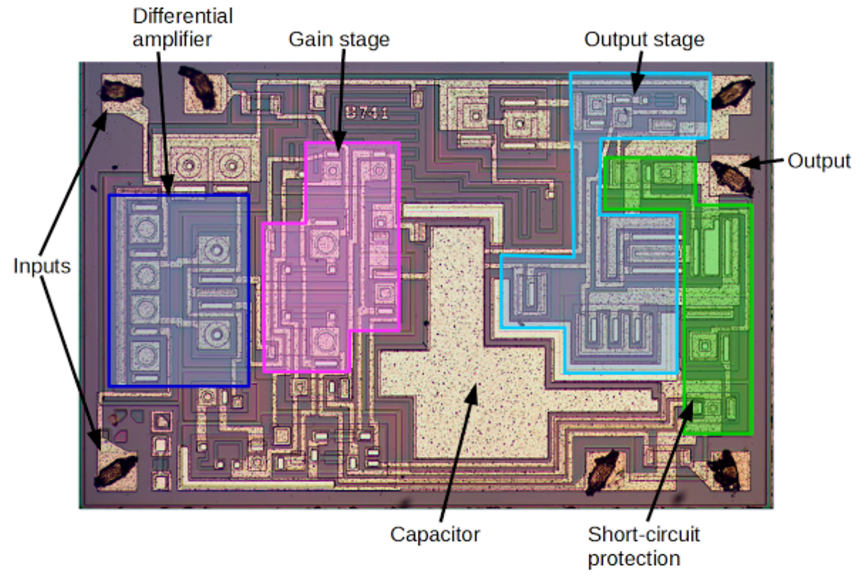
\includegraphics[height=2.5cm]{figura33.png}
			\end{center}	
		\end{column}	

	\end{columns} \\

	
		\begin{columns}
		\begin{column}{.22\textwidth}  %%<--- here			
		\begin{center}
		 
		\textbf{\scalebox{0.5}{741 Op Amp integrated circuit}}
		
		\end{center}
		\end{column}
		\begin{column}{.24\textwidth}  %%<--- here
		\begin{center}
		\textbf{ \scalebox{0.5}{741 Op Amp Pin numbers}}
		 \end{center}	
		\end{column}
		\begin{column}{.24\textwidth}  %%<--- here
		\begin{center}
		\textbf{\scalebox{0.5}{741 Op Amp schematic}}\\
		\scalebox{0.5}{\url{http://www.falstad.com/circuit/}}	
		\end{center}	
		\end{column}	
		\begin{column}{.32\textwidth}  %%<--- here
		\begin{center}
		\textbf{\scalebox{0.5}{741 Op Amp inside}}\\
		\scalebox{0.5}{\url{http://www.epanorama.net/}}	
		\end{center}	
		\end{column}	

		
		
		
		
		\end{columns}
	
	




\end{tabular}
\end{frame}
% ----------------- NOVO SLIDE --------------------------------
\begin{frame}[fragile]
\frametitle{The Operational Amplifier}
\begin{tabular}{r}

	\begin{columns}	\column{1\textwidth}
	The power supplies are used to bias the operational amplifier. In other words, the power supplies
cause certain conditions that are required for the operational amplifier to function properly.
	\end{columns} \\
	\begin{columns}
		\begin{column}{.5\textwidth}  %%<--- here
	%		\begin{center}
			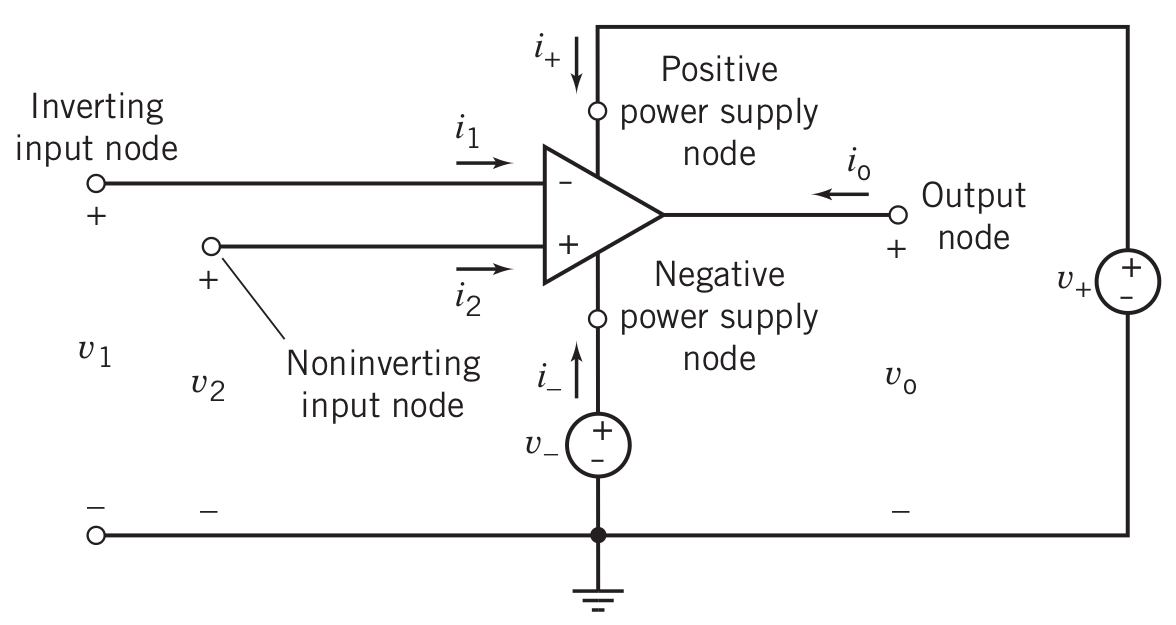
\includegraphics[height=4cm]{figura03.png}\\ 
			%	\end{center}			

		\end{column}
		\begin{column}{.5\textwidth}  %%<--- here
		
		    \begin{itemize}
		    \item[$\clubsuit$]{These power supplies tend to clutter drawings of operational amplifier circuits, making them harder to read; \newline}
		    \item[$\clubsuit$]{Consequently, the power supplies are frequently omitted from drawings that accompany explanations
of the function of operational amplifier circuits.}	
			
		  \end{itemize}
		
		
			
		\end{column}
	\end{columns} \\

	


\end{tabular}
\end{frame}
% ----------------- NOVA SECÇÂO -----------------------------
\section{Operational Amplifiers 5.2 (Sadiku)}
% ----------------- NOVO SLIDE --------------------------------
\begin{frame}[fragile]
\frametitle{Operational Amplifiers}
\begin{tabular}{r}
	\begin{columns}	\column{1\textwidth}
	An op amp is an active circuit element designed to perform mathematical operations of addition, subtraction, multiplication, division, differentiation, and integration.
\newline
	\end{columns} \\
	\begin{columns}
		\begin{column}{.5\textwidth}  %%<--- here
	%		\begin{center}
			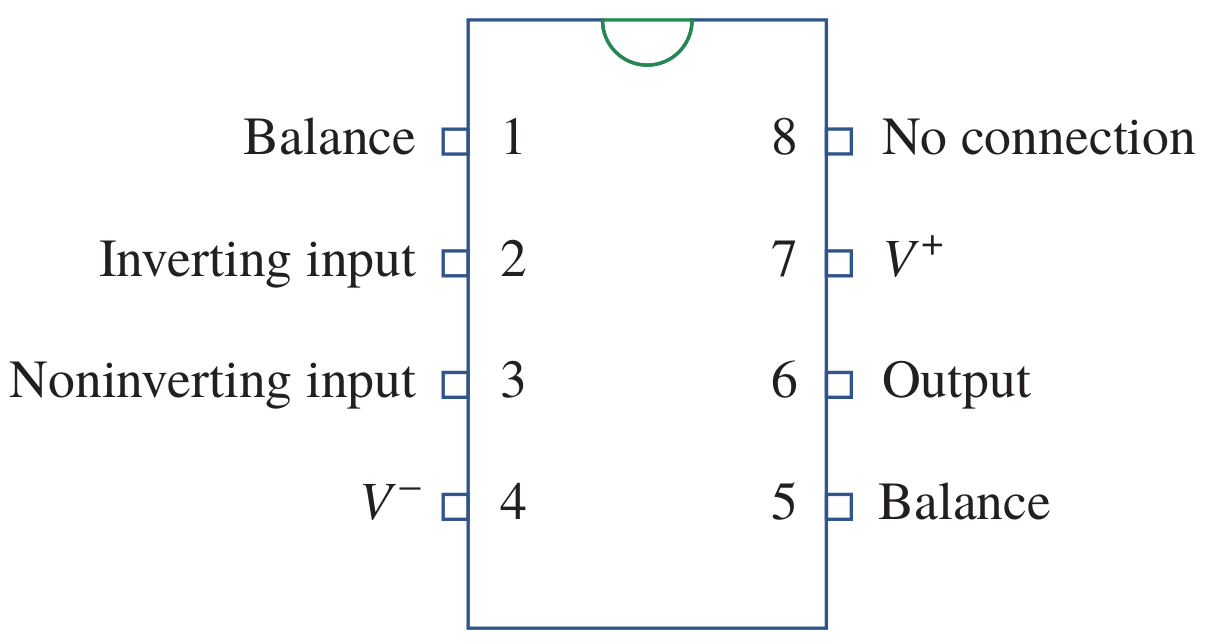
\includegraphics[height=3.5cm]{figura05.png}
			%	\end{center}			

		\end{column}
	%	\begin{column}{.2\textwidth}  %%<--- here
	%		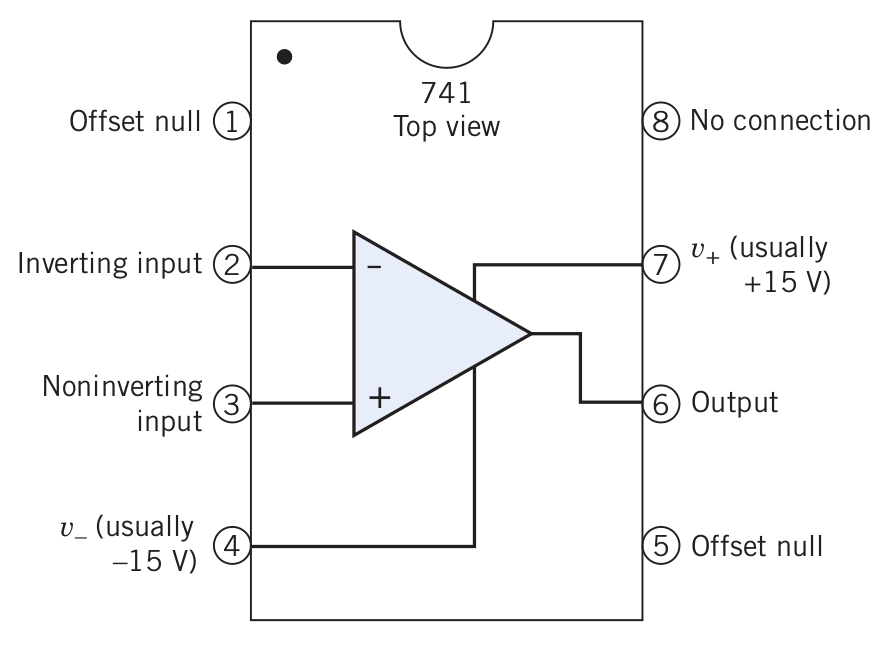
\includegraphics[height=3cm]{figura02.png}\\ (b)
	%	\end{column}
		\begin{column}{.6\textwidth}  %%<--- here
		    \begin{itemize}
		    \item[$\clubsuit$]{The inverting input, pin 2;}
		    \item[$\clubsuit$]{The noninverting input, pin 3.}	
		    \item[$\clubsuit$]{The output, pin 6.}		
		    \item[$\clubsuit$]{The positive power supply $V^{+}$, pin 7.}	
		    \item[$\clubsuit$]{The negative power supply $V^{-}$, pin 4.}		
		  \end{itemize}
		\end{column}	
	\end{columns} \\
\end{tabular}
\end{frame}

% ----------------- NOVO SLIDE --------------------------------
\begin{frame}[fragile]
\frametitle{Operational Amplifiers}
\begin{tabular}{r}
	\begin{columns}	\column{1\textwidth}
	The equivalent circuit of the nonideal op amp.

	\end{columns} \\
	\begin{columns}
		\begin{column}{.2\textwidth}  %%<--- here
		\begin{center}
			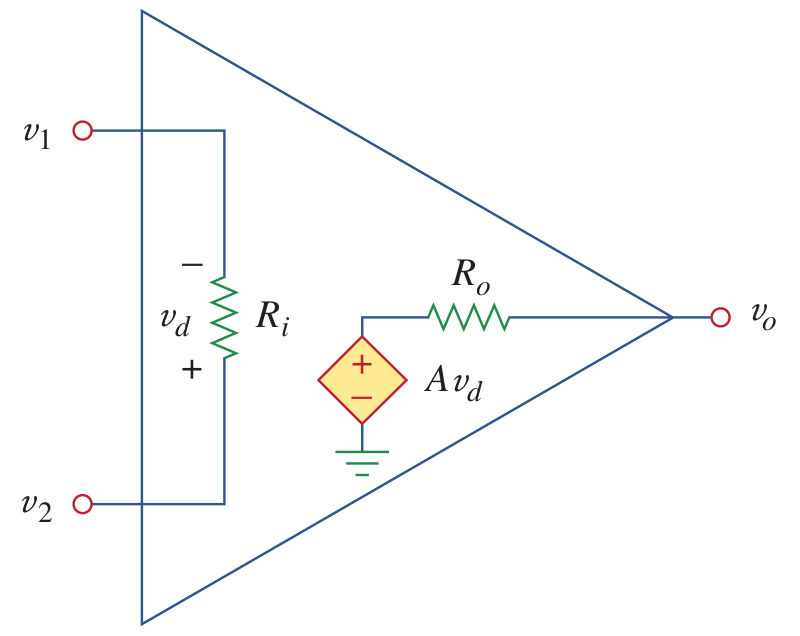
\includegraphics[height=3.2cm]{figura06.png}
			\end{center}			

		\end{column}
		\begin{column}{.7\textwidth}  %%<--- here
			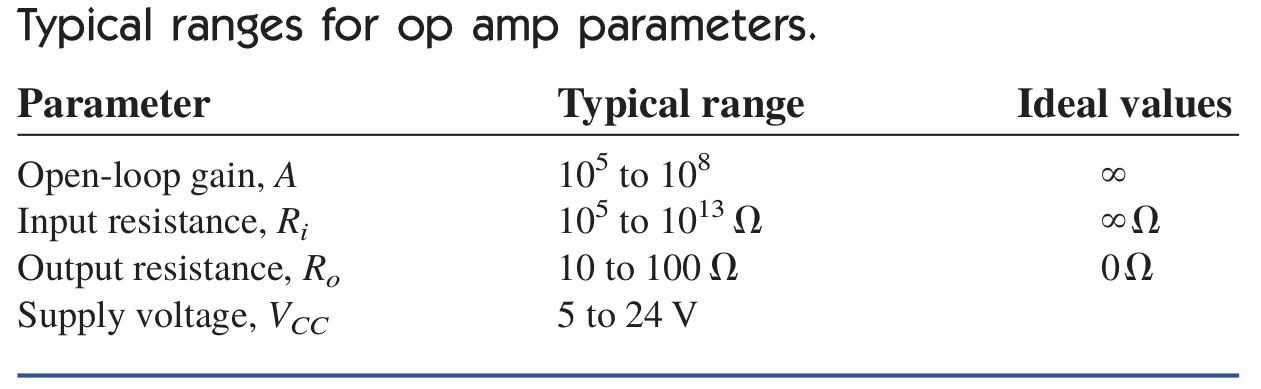
\includegraphics[height=3cm]{figura07.png}
		\end{column}
	
	\end{columns} \\
	\begin{columns}	\column{1\textwidth}
	{\newline The differential input voltage $v_{d}$ is given by $v_{d}=v_{2}-v_{1}$. The output $v_{o}$ is given by $v_{o}=Av_{d}=A(v_{2}-v_{1})$.}
	\end{columns}
	
\end{tabular}
\end{frame}
% ----------------- NOVO SLIDE --------------------------------
\begin{frame}[fragile]
\frametitle{Operational Amplifiers}
\begin{tabular}{r}
	\begin{columns}	\column{1\textwidth}
	A practical limitation of the op amp is that the magnitude of its output voltage cannot exceed |$V_{CC}$|.
\newline
	\end{columns} \\
	\begin{columns}
		\begin{column}{.4\textwidth}  %%<--- here
	%		\begin{center}
			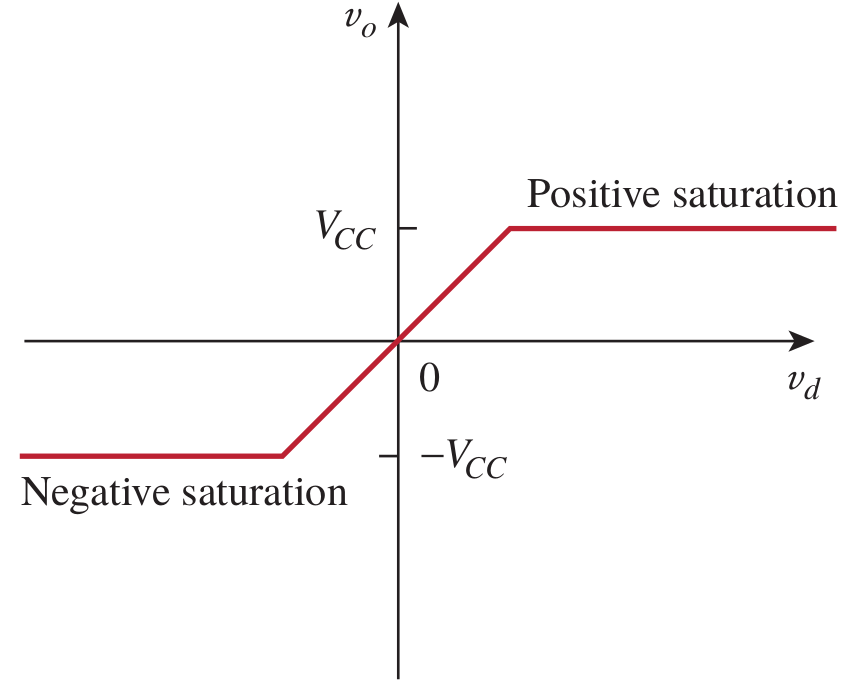
\includegraphics[height=4.5cm]{figura10.png}
			%	\end{center}			

		\end{column}
	%	\begin{column}{.2\textwidth}  %%<--- here
	%		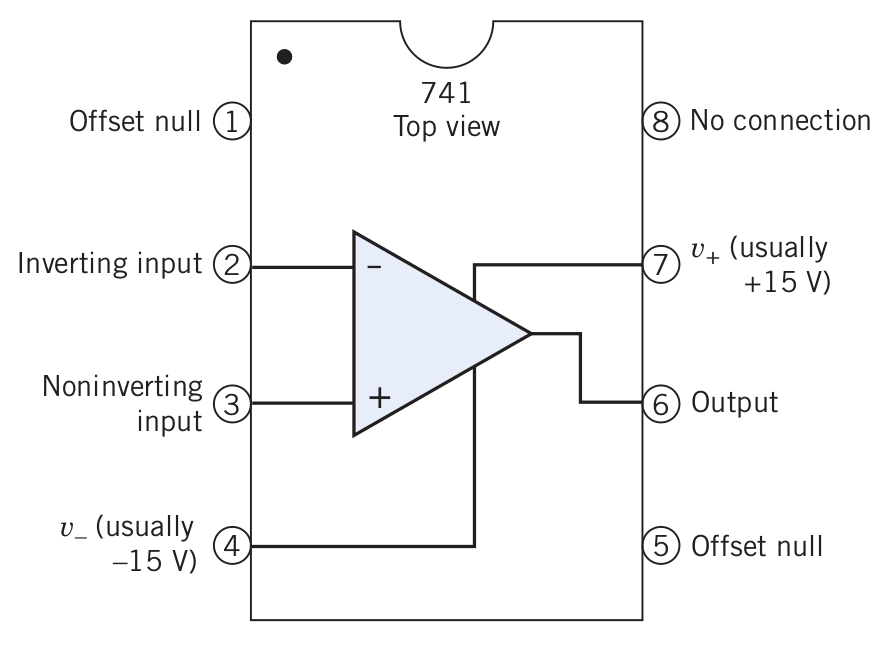
\includegraphics[height=3cm]{figura02.png}\\ (b)
	%	\end{column}
		\begin{column}{.6\textwidth}  %%<--- here
		    \begin{itemize}
		    \item[$\clubsuit$]{Positive saturation, $v_{o}=V_{CC}$;\newline}
		    \item[$\clubsuit$]{Linear region, $-V_{CC} \leq v_{o}= Av_{d} \leq V_{CC}$;\newline}	
		    \item[$\clubsuit$]{Negative saturation, $v_{o}=-V_{CC}$.}			
		  \end{itemize}
		\end{column}	
	\end{columns} \\
\end{tabular}
\end{frame}

% ----------------- NOVO SLIDE --------------------------------
\begin{frame}[fragile]
\frametitle{Operational Amplifiers}
\begin{tabular}{r}
	
		\begin{columns}
		\begin{column}{1\textwidth}  %%<--- here
		\textbf{Example 5.1} - A 741 op amp has an open-loop voltage gain of $2.10^{5}$, input resis-
tance of $2M\Omega$, and output resistance of $50 \Omega$. Find the closed-loop gain $\frac{v_{o}}{v_{s}}$ and determine current $i$ when $v_{s}=2V$.\\
		\begin{center}
    			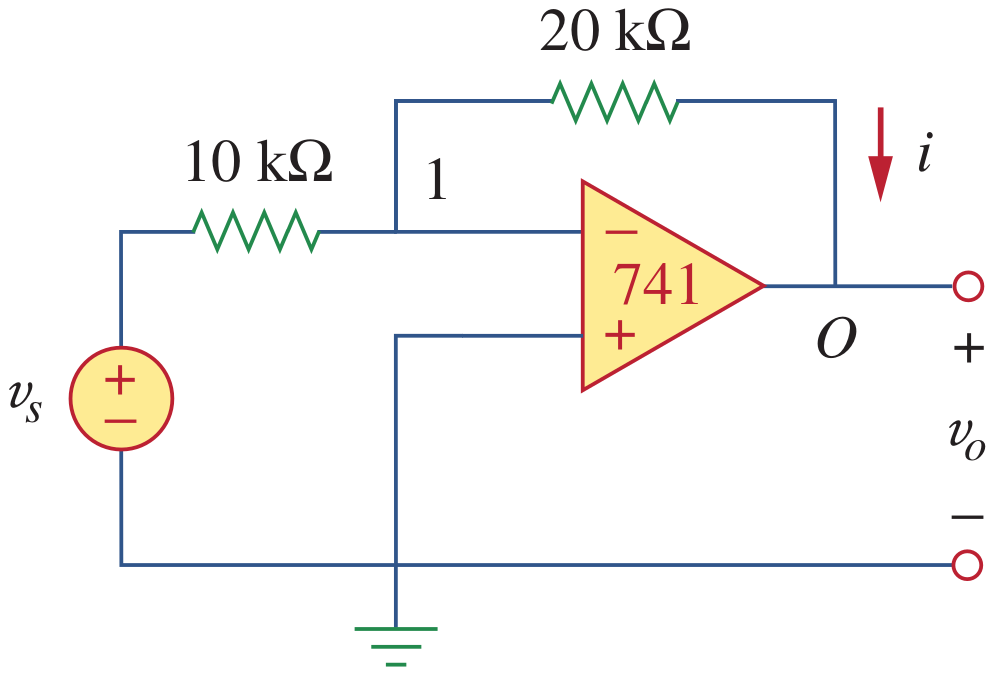
\includegraphics[height=.2\textwidth]{figura08.png} {. \ . \ . \ . \ . \ . \ .}
    			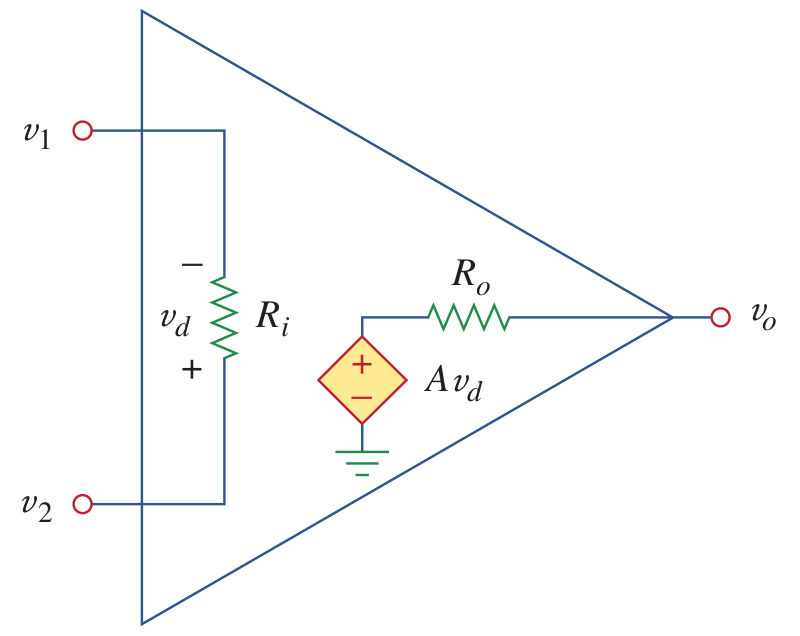
\includegraphics[height=.2\textwidth]{figura06.png}	
		\end{center}
	
		\scalebox{0.8}{Answer: $ \frac{v_{o}}{v_{s}}=-1.9999698 \ and \  i=0.19999mA $}
		\end{column}
	\end{columns}
	
	
	
\end{tabular}
\end{frame}

%----------------- NOVO SLIDE --------------------------------
\begin{frame}[fragile]
\frametitle{Operational Amplifiers}
\begin{tabular}{r}
	
		\begin{columns}
		\begin{column}{1\textwidth}  %%<--- here
		\textbf{Practice Problem 5.1} - If the same 741 op amp in Example 5.1 is used in the circuit below, calculate the closed-loop gain $\frac{v_{o}}{v_{s}}$. Find $i_{o}$ when $v_{s}=2V$.\\
		\begin{center}
    			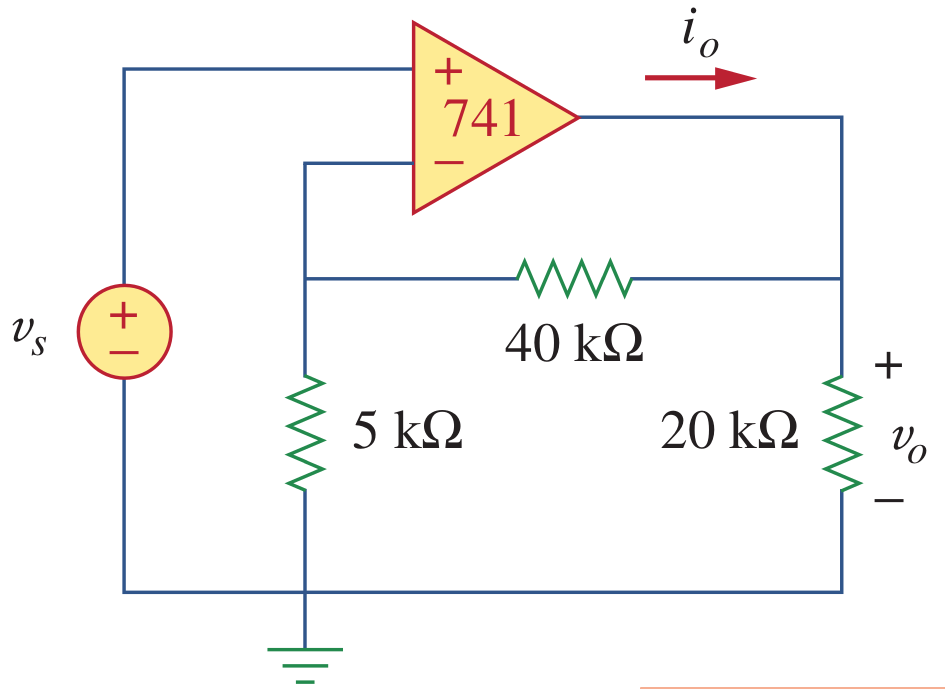
\includegraphics[height=.2\textwidth]{figura09.png} {. \ . \ . \ . \ . \ . \ .}
    			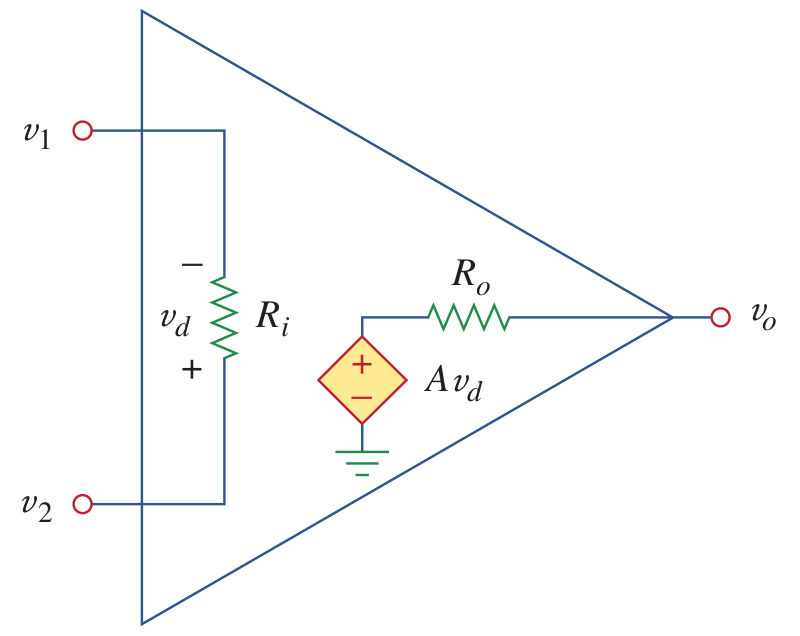
\includegraphics[height=.2\textwidth]{figura06.png}	
		\end{center}
	
		\scalebox{0.8}{Answer: $ \frac{v_{o}}{v_{s}}=9.00041 \ and \  i=0.657mA $}
		\end{column}
	\end{columns}
	
	
	
\end{tabular}
\end{frame}






% ----------------- NOVA SECÇÂO -----------------------------
\section{The Ideal Operational Amplifier (6.3)}
% ----------------- NOVO SLIDE --------------------------------
\begin{frame}[fragile]
\frametitle{The Ideal Operational Amplifier}
\begin{tabular}{r}
	\begin{columns}	\column{1\textwidth}
	The ideal operational amplifier is a simple
model of an operational amplifier that is linear. 

	\end{columns} \\
	\begin{columns}
		\begin{column}{.3\textwidth}  %%<--- here
	%		\begin{center}
			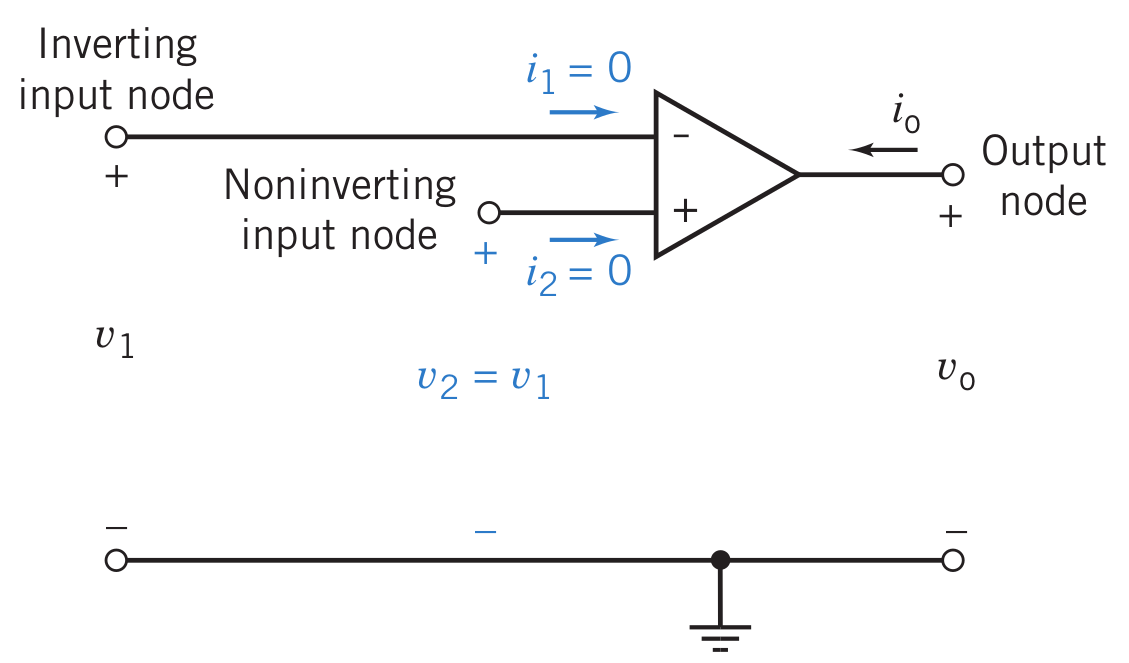
\includegraphics[height=3cm]{figura04.png}
			%	\end{center}			

		\end{column}
		\begin{column}{.6\textwidth}  %%<--- here
		
		  \begin{itemize}
		    \item[$\clubsuit$]{The currents into the input terminals of an ideal
operational amplifier are zero ($i_{1}=i_{2}=0$).\newline}
		    \item[$\clubsuit$]{The node voltages at the input nodes of an ideal operational amplifier are equal ($A=\infty \ and \ v_{1}=v_{2}$).\newline}	
		  		
		  \end{itemize}
		
			 
		\end{column}
	\end{columns} \\

	\begin{columns}	\column{1\textwidth}
	{\newline The ideal operational amplifier is characterized by restrictions on its input currents and voltages.}
	\end{columns}





\end{tabular}
\end{frame}
% ----------------- NOVA SECÇÂO -----------------------------
\section{Nodal Analysis of Circuits Containing Ideal Operational Amplifiers (6.4)}
% ----------------- NOVO SLIDE --------------------------------
\begin{frame}[fragile]
\frametitle{Nodal Analysis of Circuits Containing Ideal Operational Amplifiers}
\begin{tabular}{r}
 
\begin{columns}	\column{1\textwidth}
	

	\end{columns} \\
	\begin{columns}
		\begin{column}{.5\textwidth}  %%<--- here
	%		\begin{center}
	{\newline \textbf{EXEMPLE 6.4.1} Use node equations to analyze this circuit and determine $v_{o}$ in terms of the two source
voltages $v_{a}$ and $v_{b}$ .}\\
			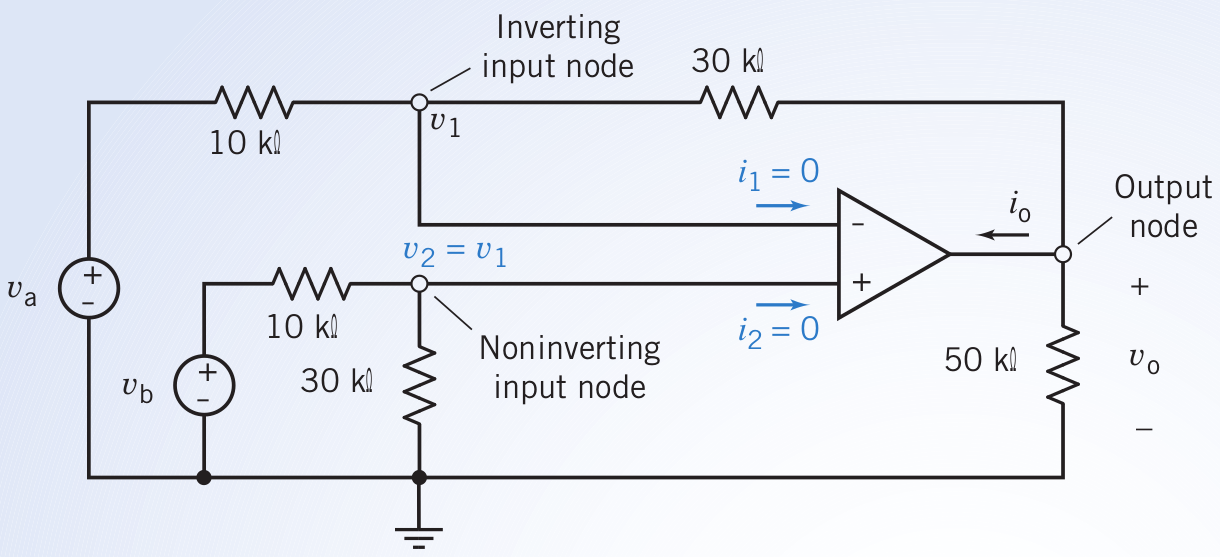
\includegraphics[height=3cm]{figura11.png}\\
			
			%	\end{center}			

		\end{column}
		\begin{column}{.5\textwidth}  %%<--- here
		There are three things to remember:\newline
		  \begin{itemize}
		    \item[$\clubsuit$]{The node voltages at the input nodes of ideal operational amplifiers are equal.}
		    \item[$\clubsuit$]{The currents in the input leads of an ideal operational amplifier are zero.}	
		    \item[$\clubsuit$]{The output current of the operational amplifier is not zero.}		
		  \end{itemize}
		
			 
		\end{column}
	\end{columns} \\
\begin{columns}
		\begin{column}{1\textwidth}  %%<--- here
		\newline	\scalebox{0.6}{Answer: $v_{o}=3(v_{b}-v_{a}) $} 
		\end{column}
	\end{columns} \\

\end{tabular}
\end{frame}
% ----------------- NOVO SLIDE --------------------------------
\begin{frame}[fragile]
\frametitle{Analysis of a Bridge Amplifier}
\begin{tabular}{r}


		\begin{columns}
		\begin{column}{1\textwidth}  %%<--- here
		\textbf{Example 6.4.2} - Determine the output voltage $v_{o}$ in terms of the source voltage $v_{s}$ .\\
		\begin{center}
    			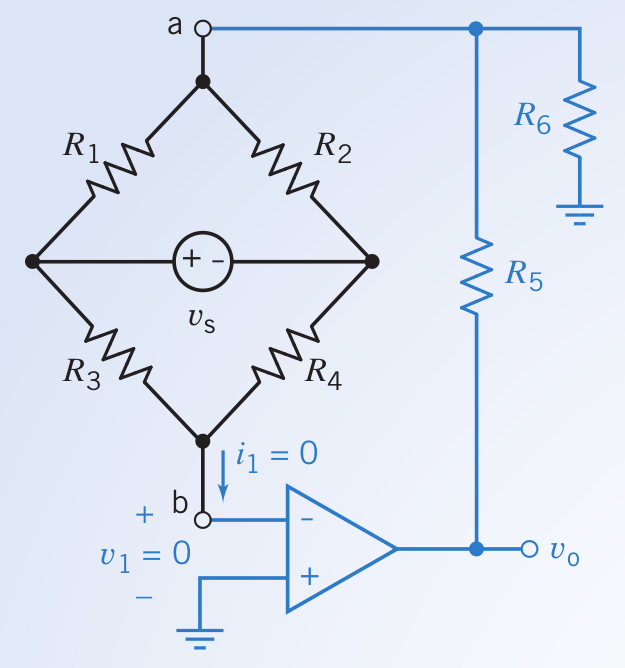
\includegraphics[height=.3\textwidth]{figura12.png}	
		\end{center}
	
		\scalebox{0.8}{Answer: $v_{o}=(1+\frac{R_{5}}{R_{6}})(\frac{R_{2}}{R_{1}+R_{2}}-\frac{R_{4}}{R_{3}+R_{4}})v_{s}$}
		\end{column}
	\end{columns}
	

\end{tabular}
\end{frame}
% ----------------- NOVO SLIDE --------------------------------
\begin{frame}[fragile]
\frametitle{Nodal Analysis}
\begin{tabular}{r}


	
	
	\begin{columns}
		\begin{column}{1\textwidth}  %%<--- here
		 \textbf{Problem 6.4.1} - Determine the node voltages for the circuit shown in Figure below. \newline
		\end{column}
  \end{columns}\\

    \begin{columns}
		\begin{column}{.5\textwidth}  %%<--- here
		
		%    \begin{center}
    			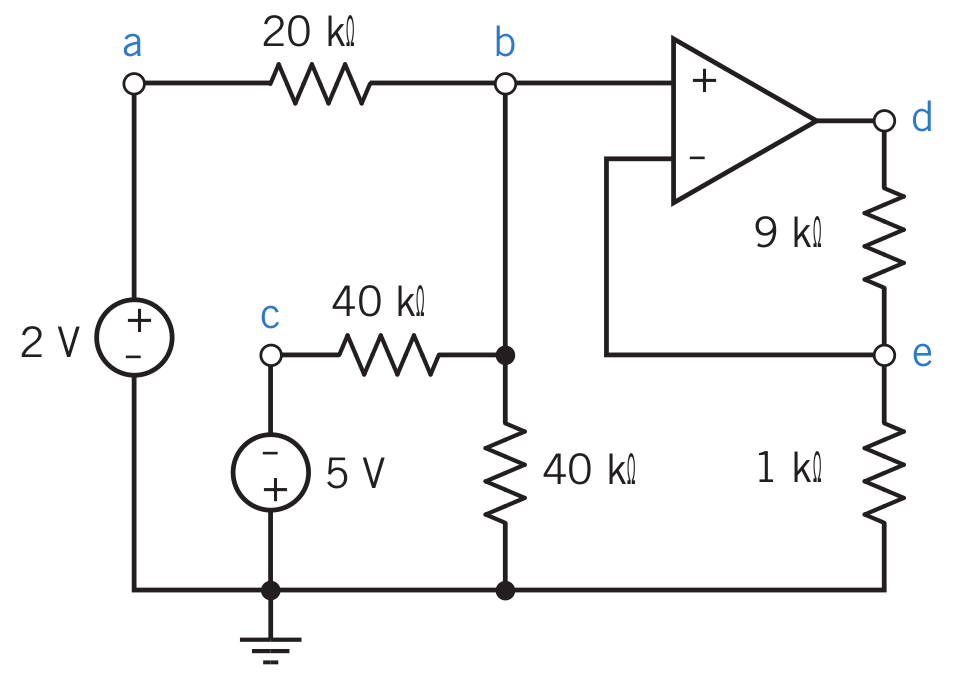
\includegraphics[height=.6\textwidth]{figura13.png}
    			
		 %   \end{center}
		\end{column}
		\begin{column}{.5\textwidth}  %%<--- here
		
		  %  \begin{center}
    			
    			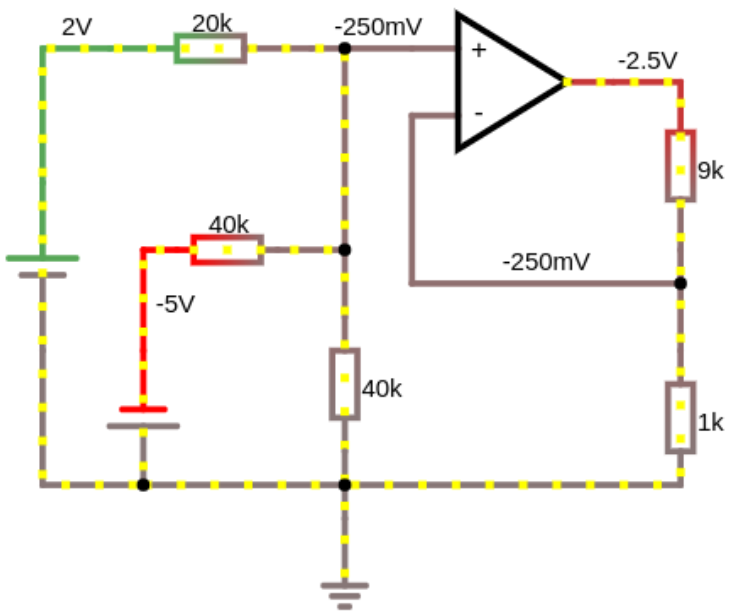
\includegraphics[height=.6\textwidth]{figura31.png}
    			
		   % \end{center}
		\end{column}
  \end{columns}\\
\newline \newline
	
 \begin{columns}
		\begin{column}{.5\textwidth}  %%<--- here
		 \scalebox{0.6}{Answer: $v_{a}=2V, v_{b}=-0.25V, v_{c}=-5V, v_{d}=-2.5V, \ and \ v_{e}=-0.25V.  $}
		\end{column}
 		\begin{column}{.5\textwidth}  %%<--- here
		  \scalebox{0.8}{\url{http://www.falstad.com/circuit/}}
		\end{column}
  \end{columns}\\
	
	
	
	
	
	
	
	
	
	
	
	
	

\end{tabular}
\end{frame}
% ----------------- NOVO SLIDE --------------------------------
\begin{frame}[fragile]
\frametitle{Nodal Analysis}
\begin{tabular}{r}


	
		\begin{columns}
		\begin{column}{1\textwidth}  %%<--- here
		\textbf{Problem 6.4.5} - Express the outputs as functions of the inputs and the resistor resistances.\\
		\begin{center}
    			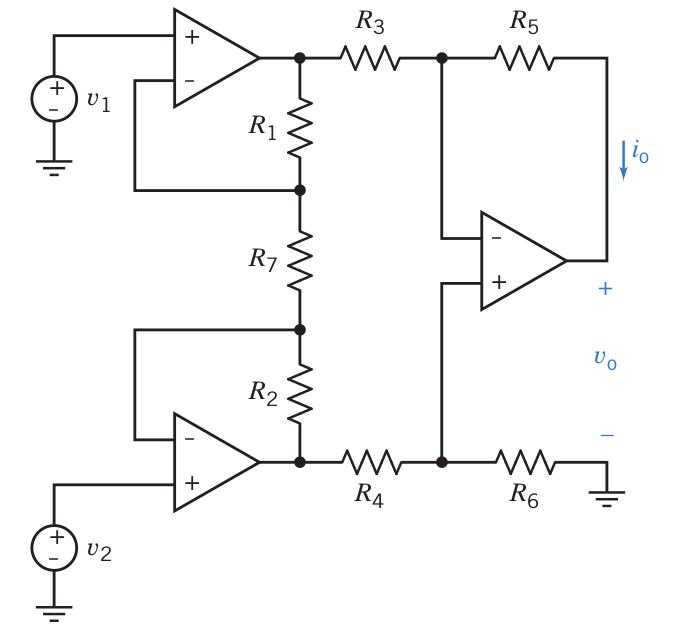
\includegraphics[height=.35\textwidth]{figura15.png}	
		\end{center}
	
		%\scalebox{0.8}{Answer: $v_{a}=2V, v_{b}=-0.25V, v_{c}=-5V, v_{d}=-2.5V, \ and \ v_{e}=-0.25V.  $}
		\end{column}
	\end{columns}
	

\end{tabular}
\end{frame}
% ----------------- NOVO SLIDE --------------------------------
\begin{frame}[fragile]
\frametitle{Nodal Analysis}
\begin{tabular}{r}


\begin{columns}
		\begin{column}{1\textwidth}  %%<--- here
		 \textbf{Problem 6.4.6} - Determine the node voltages for the circuit shown in Figure below. \newline
		\end{column}
  \end{columns}\\

    \begin{columns}
		\begin{column}{.5\textwidth}  %%<--- here
		
		%    \begin{center}
    			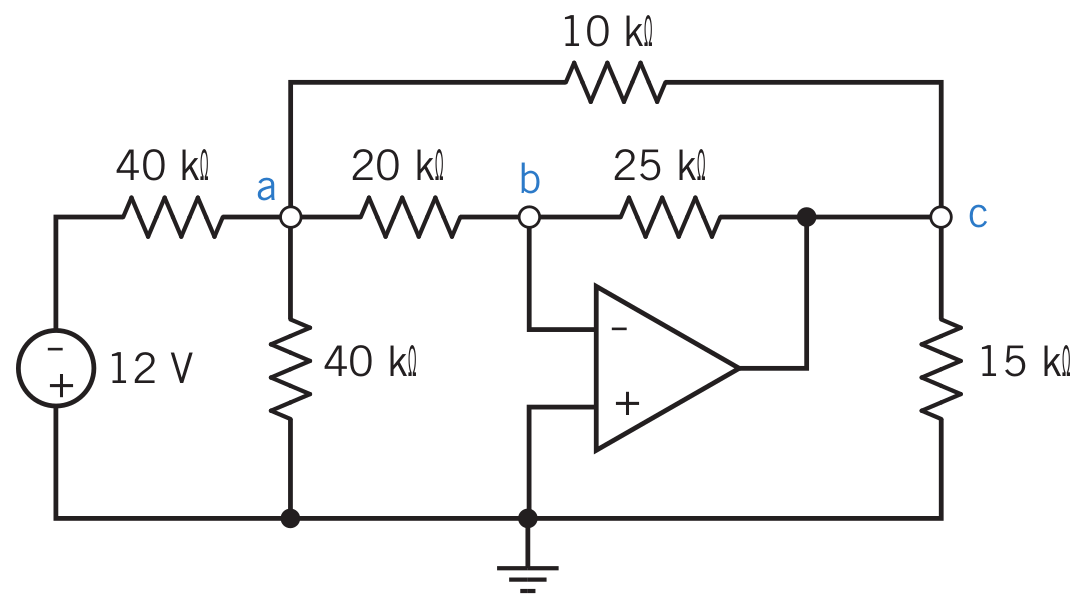
\includegraphics[height=.6\textwidth]{figura14.png}
    			
		 %   \end{center}
		\end{column}
		\begin{column}{.5\textwidth}  %%<--- here
		
		  %  \begin{center}
    			
    			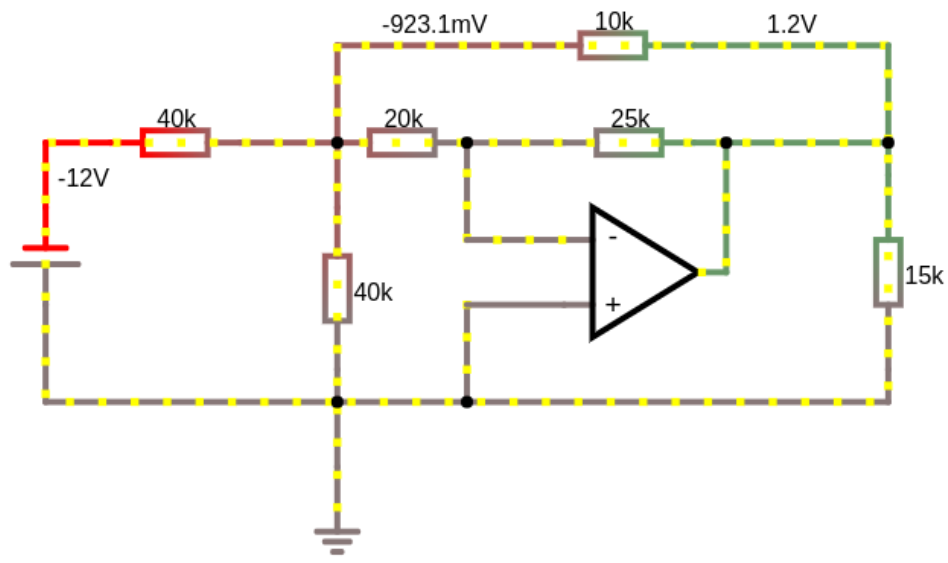
\includegraphics[height=.6\textwidth]{figura30.png}
    			
		   % \end{center}
		\end{column}
  \end{columns}\\
\newline \newline
	
 \begin{columns}
		\begin{column}{.5\textwidth}  %%<--- here
		  \scalebox{0.6}{Answer: $v_{a}=-0.923V, v_{b}=0V \ and \ v_{c}=1.154V.$}
		\end{column}
 		\begin{column}{.5\textwidth}  %%<--- here
		  \scalebox{0.8}{\url{http://www.falstad.com/circuit/}}
		\end{column}
  \end{columns}\\
	

\end{tabular}
\end{frame}

% ----------------- NOVA SECÇÂO -----------------------------
\section{Design Using Operational Amplifiers (6.5)}
% ----------------- NOVO SLIDE --------------------------------
\begin{frame}[fragile]
\frametitle{Standard Operational Amplifier Circuits}
\begin{tabular}{r}

		\begin{columns}	\column{1\textwidth}
 One of the early applications of operational amplifiers was to build circuits that performed mathematical
operations.	\newline 
	\end{columns} \\


	\begin{columns}
		\begin{column}{.33\textwidth}  %%<--- here
		\begin{center}
			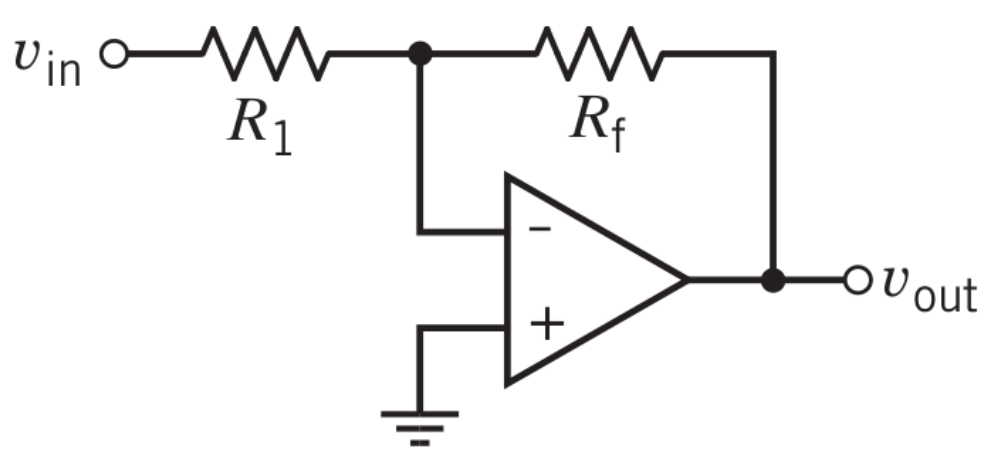
\includegraphics[height=2.0cm]{figura16.png}
			\end{center}			

		\end{column}
		\begin{column}{.33\textwidth}  %%<--- here
			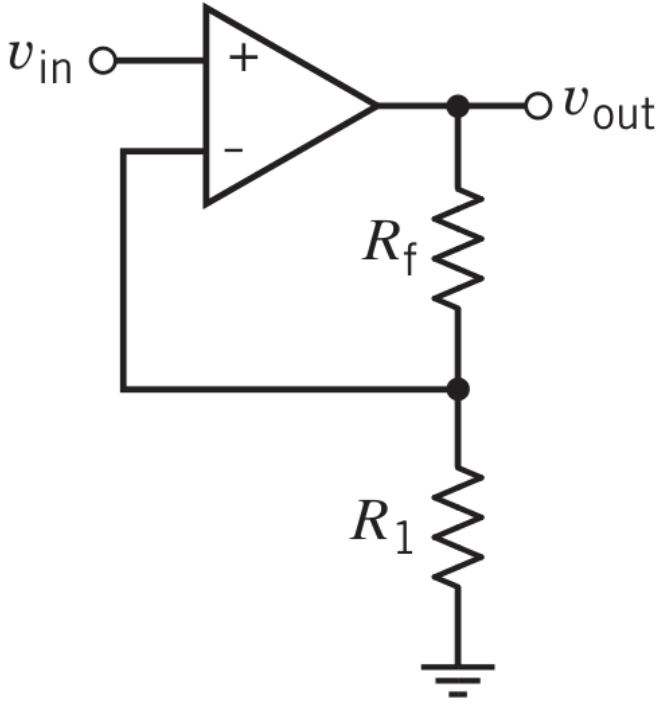
\includegraphics[height=3.0cm]{figura17.png}
		\end{column}
		\begin{column}{.33\textwidth}  %%<--- here
			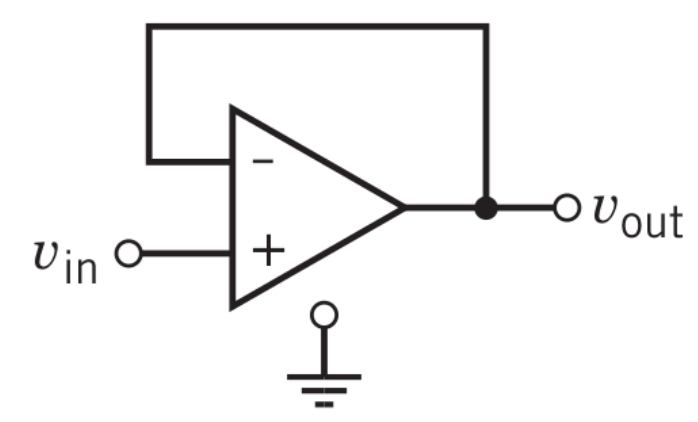
\includegraphics[height=2.0cm]{figura18.png}
		\end{column}
	
	\end{columns} \\
	
	
		\begin{columns}
		\begin{column}{.33\textwidth}  %%<--- here
		\begin{center}
		      \textbf{\scalebox{0.8}{ $v_{out}=-\frac{R_{f}}{R_{1}}v_{in}$}}
		      \textbf{\scalebox{0.8}{\textit{Inverting amplifier}}} 

		\end{center}			

		\end{column}
		\begin{column}{.33\textwidth}  %%<--- here
			\begin{center}
			\textbf{\scalebox{0.8}{ $v_{out}=-\frac{R_{f}}{R_{1}}v_{in}$}}
			\textbf{\scalebox{0.8}{ \textit{Noinverting amplifier}}} 

			\end{center}
		\end{column}
		\begin{column}{.33\textwidth}  %%<--- here
			\begin{center}
			\textbf{\scalebox{0.8}{ $v_{out}=v_{in}$}} \\
			\textbf{\scalebox{0.8}{\textit{Voltage follower}}} \\ \textbf{\scalebox{0.8}{\textit{(buffer Amplifier)}}}

			\end{center}
		\end{column}
	
	\end{columns} \\
	
\end{tabular}
\end{frame}
% ----------------- NOVO SLIDE --------------------------------
\begin{frame}[fragile]
\frametitle{Standard Operational Amplifier Circuits}
\begin{tabular}{r}

	\begin{columns}	\column{1\textwidth}
 Many of the operational amplifier circuits that perform mathematical operations are used so often that they have been
given names. 	\newline
	\end{columns} \\
	
	

	\begin{columns}
		\begin{column}{.33\textwidth}  %%<--- here
		\begin{center}
			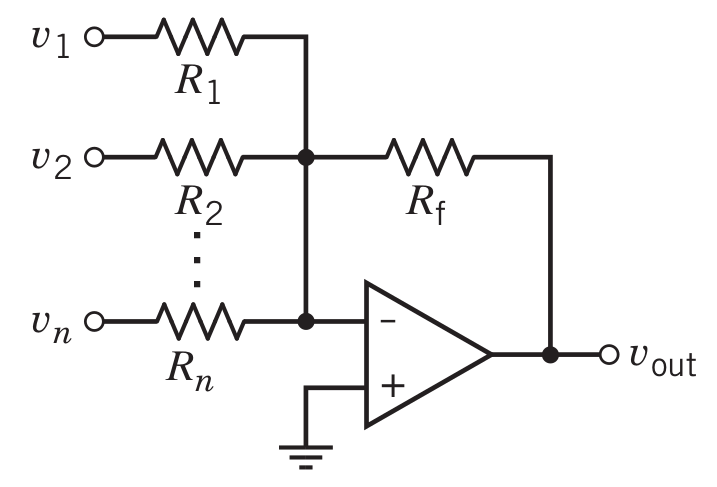
\includegraphics[height=3cm]{figura19.png}
			\end{center}			

		\end{column}
		\begin{column}{.33\textwidth}  %%<--- here
			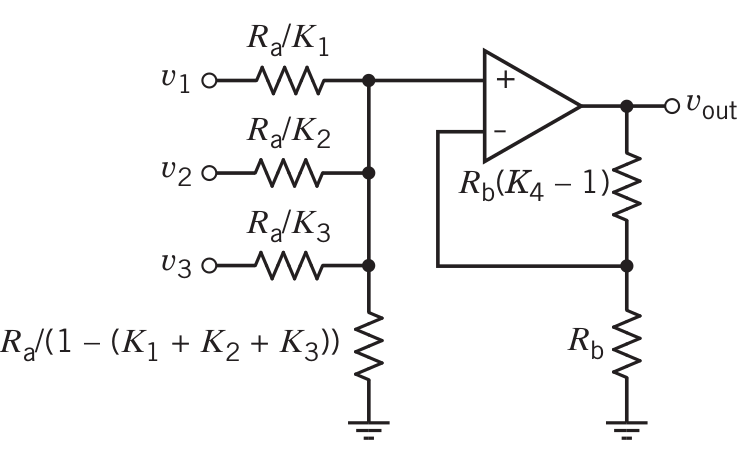
\includegraphics[height=3.2cm]{figura20.png}
		\end{column}
		\begin{column}{.28\textwidth}  %%<--- here
			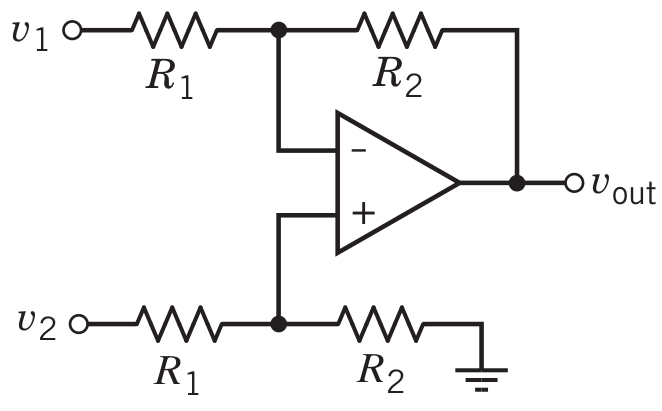
\includegraphics[height=2.5cm]{figura21.png}
		\end{column}
	
	\end{columns} \\
	
			\begin{columns}
		\begin{column}{.33\textwidth}  %%<--- here
		\begin{center}
			\textbf{\scalebox{0.8}{$v_{out}=-(\frac{R_{f}}{R_{1}}v_{1}+\frac{R_{f}}{R_{2}}v_{2}+...+\frac{R_{f}}{R_{n}}v_{n})$}}
			\textbf{\scalebox{0.8}{ \textit{Summing amplifier}}} \\
		
		\end{center}			

		\end{column}
		\begin{column}{.33\textwidth}  %%<--- here
			\begin{center}
			\textbf{\scalebox{0.8}{$v_{out}=-K_{4}(K_{1}v_{1}+K_{2}v_{2}+K_{3}v_{3})$}}
			\textbf{\scalebox{0.8}{ \textit{Noinverting summing amplifier}}} \\

			\end{center}
		\end{column}
		\begin{column}{.33\textwidth}  %%<--- here
			\begin{center}
			\textbf{\scalebox{0.8}{$v_{out}=\frac{R_{2}}{R_{1}}(v_{2}-v_{1})$}}
			\textbf{\scalebox{0.8}{\textit{Difference amplifier}}} \\

			\end{center}
		\end{column}
	
	\end{columns} \\
	

\end{tabular}
\end{frame}
% ----------------- NOVO SLIDE --------------------------------
\begin{frame}[fragile]
\frametitle{Standard Operational Amplifier Circuits}
\begin{tabular}{r}

	
	\begin{columns}	\column{1\textwidth}
These names are part of an electrical engineer’s vocabulary. 	\newline 
	\end{columns} \\

	
		
	\begin{columns}
		\begin{column}{.33\textwidth}  %%<--- here
		\begin{center}
			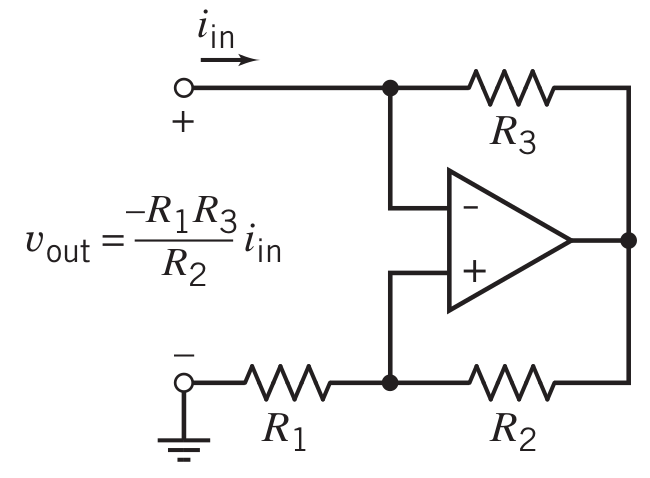
\includegraphics[height=2.5cm]{figura22.png}
			\end{center}			

		\end{column}
		\begin{column}{.33\textwidth}  %%<--- here
			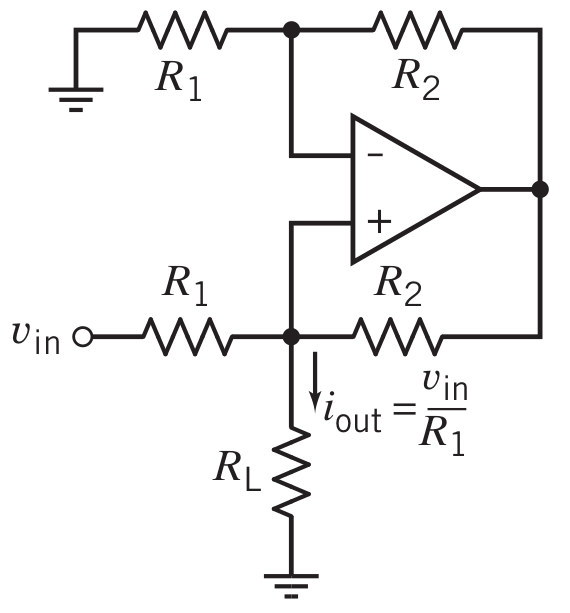
\includegraphics[height=3.3cm]{figura23.png}
		\end{column}
		\begin{column}{.33\textwidth}  %%<--- here
			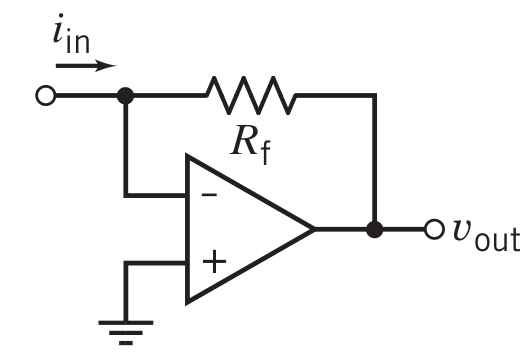
\includegraphics[height=2.5cm]{figura24.png}
		\end{column}
	
	\end{columns} \\
	
	  \begin{columns}
		\begin{column}{.33\textwidth}  %%<--- here
		\begin{center}
			\textbf{\scalebox{0.8}{$R_{in}=\frac{v_{in}}{i_{in}}=-\frac{R_{1}R_{3}}{R_{2}}$}}
			\textbf{\scalebox{0.8}{\textit{Negative resistanse convertor}}}

		\end{center}			

		\end{column}
		\begin{column}{.33\textwidth}  %%<--- here
			\begin{center}
			\textbf{\scalebox{0.8}{$v_{out}=-R_{f}i_{in}$}}
			\textbf{\scalebox{0.8}{ \textit{Current-to-voltage converter}}} 

			\end{center}
		\end{column}
		\begin{column}{.33\textwidth}  %%<--- here
		\begin{center}
		
		\textbf{\scalebox{0.8}{$i_{out}=\frac{v_{in}}{R_{1}}$}}\\
		\textbf{\scalebox{0.8}{\textit{Voltage-controlled}}} \\
		\textbf{\scalebox{0.8}{\textit{current source (VCCS)}}} 
		

	
		
		
		\end{center}
		\end{column}
	
	\end{columns} \\

\end{tabular}
\end{frame}

% ----------------- NOVO SLIDE --------------------------------
\begin{frame}[fragile]
\frametitle{Design Using Operational Amplifiers}
\begin{tabular}{r}

 
		 \begin{columns}
		\begin{column}{1\textwidth}  %%<--- here
			
		\begin{center}	
			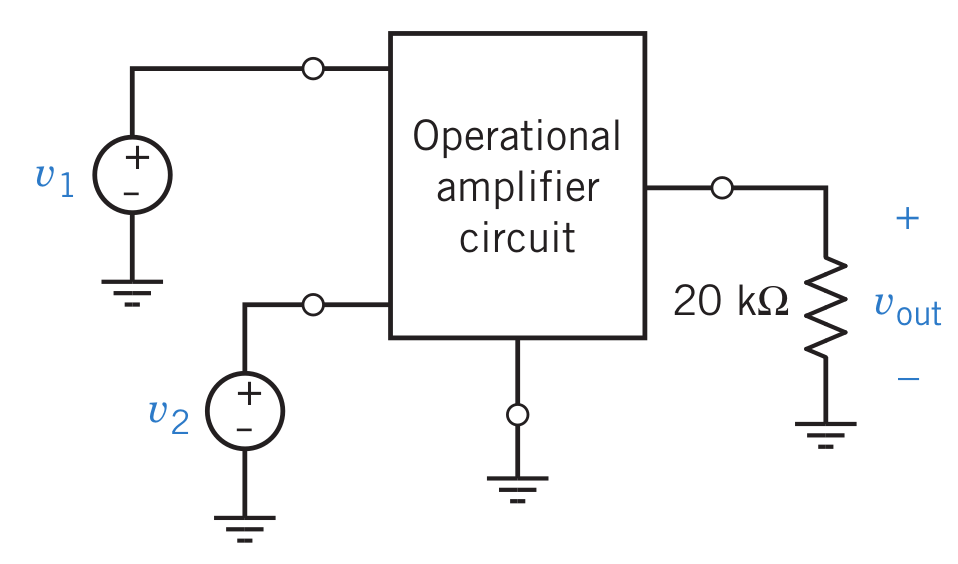
\includegraphics[height=3.5cm]{figura26.png}
		\end{center}
		\end{column}
	
	\end{columns} \\

	    \begin{columns}
		\begin{column}{1\textwidth}
		
		\textbf{Problem 6.5-4} - Design the operational amplifier circuit in Figure above so that. \\
	
	
		$v_{out}=5(v_{1}-v_{2}) $
		
		
		\end{column}
	
	
	
	
	
	\end{columns}\\
		
		    \begin{columns}
		\begin{column}{1\textwidth}
		
		\textbf{Problem 6.5-5} - Design the operational amplifier circuit in Figure above so that. \\
	
		
		$v_{out}=5v_{1}-2v_{2} $
		
		
		\end{column}
	    \end{columns}\\
		
		 
		 
  
\end{tabular}
\end{frame}



% ----------------- NOVO SLIDE --------------------------------
\begin{frame}[fragile]
\frametitle{Design Using Operational Amplifiers}
\begin{tabular}{r}
	    \begin{columns}
		\begin{column}{1\textwidth}
		\textbf{Problem 6.5-11} - The circuit shown in Figure below is called a Howland current source. It has one input, $v_{in}$, and one output,
$i_{out}$. \\
		\end{column}
	  \end{columns}\\
		\begin{columns}
		  \begin{column}{.5\textwidth}  %%<--- here
		    \begin{center}
    	  		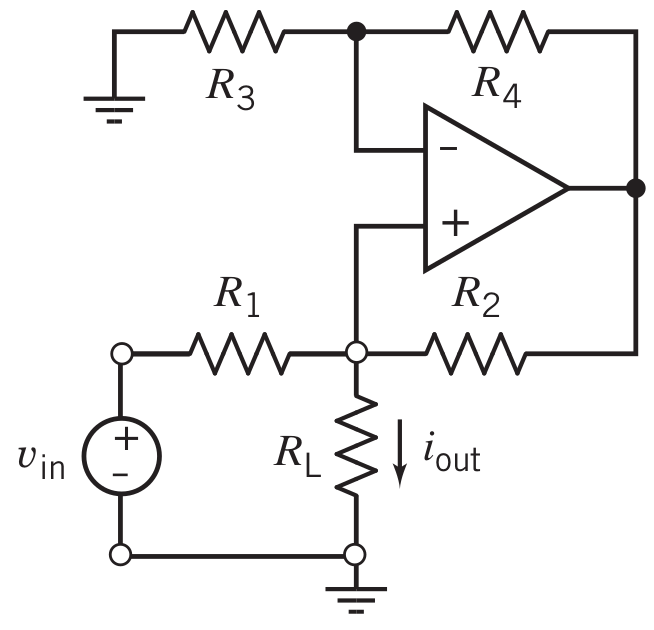
\includegraphics[height=.6\textwidth]{figura25.png}	
		    \end{center}
		\end{column}
		
	      \begin{column}{.5\textwidth}  %%<--- here
	
		Show that when the resistances are chosen so that $R_{2}R_{3} = R_{1} R_{4}$, the output is related to the input by the equation $i_{out}=\frac{v_{in}}{R_{1}}$.
	      \end{column}
	
	
	
	
	
	\end{columns}
	

	
\end{tabular}
\end{frame}



% ----------------- NOVA SECÇÂO -----------------------------
\section{Operational Amplifier Circuits and Linear Algebraic Equations (6.6)}
% ----------------- NOVO SLIDE --------------------------------
\begin{frame}[fragile]
\frametitle{Operational Amplifier Circuits and Linear Algebraic Equations}
\begin{tabular}{r}
	 \begin{columns}
		\begin{column}{1\textwidth}
		This section describes a procedure for designing operational amplifier circuits to implement linear algebraic 
		equations. For example, the equation $z=4x-5y+2$ will be represented by $v_{z}=4v_{x}-5v_{y}+2$, where $v_{z}, v_{x}$  and  $v_{y}$ are voltages.
		\end{column}
	\end{columns}\\

	\begin{columns}
	      \begin{column}{.3\textwidth}  %%<--- here
		\begin{center}
		  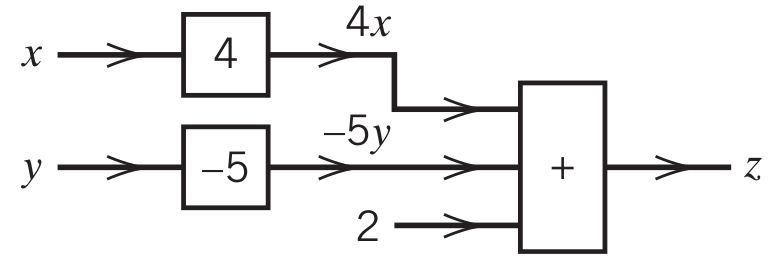
\includegraphics[height=.35\textwidth]{figura27.png}	
		\end{center}
	      \end{column}
	      \begin{column}{.1\textwidth}  %%<--- here
		\begin{center}
		  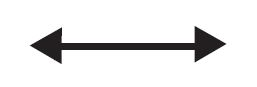
\includegraphics[height=.4\textwidth]{figura29.JPG}	
		\end{center}
	      \end{column}	
	      \begin{column}{.5\textwidth}  %%<--- here
		\begin{center}
		  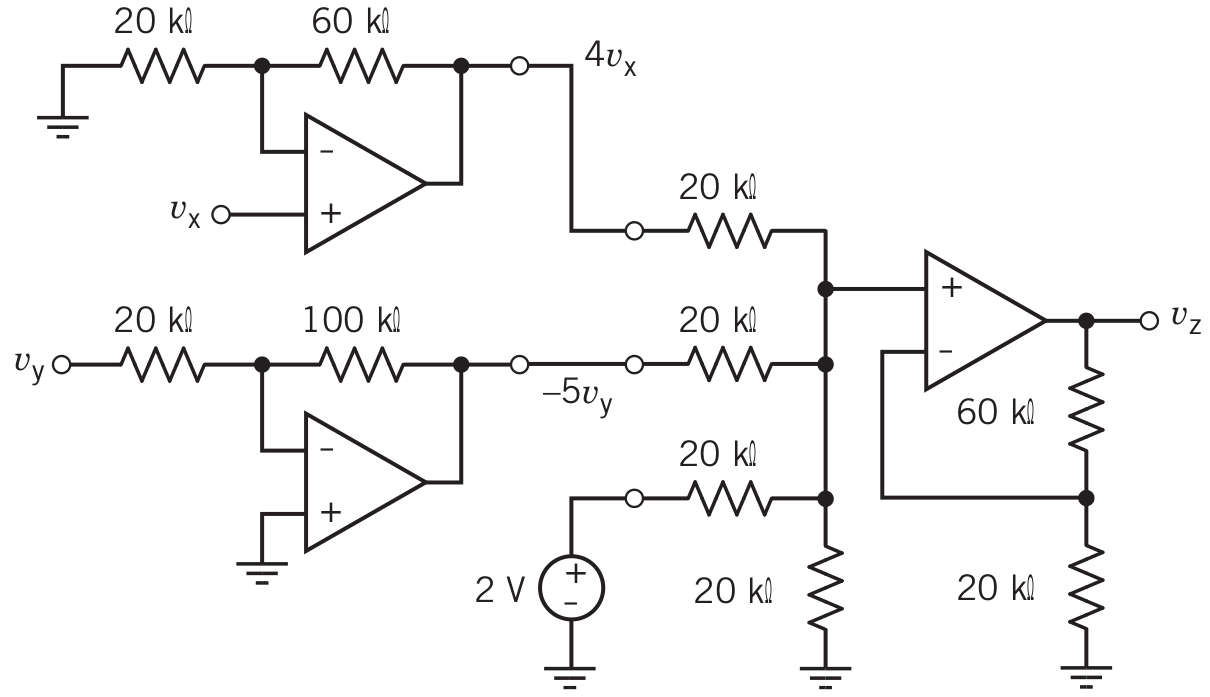
\includegraphics[height=.5\textwidth]{figura28.png}	
		\end{center}
	      \end{column}	
		
	\end{columns}\\
	 \begin{columns}
		\begin{column}{1\textwidth}
		\newline \textbf{A voltage or current that is used to represent something is called a signal.}
		\end{column}
	\end{columns}\\
\end{tabular}
\end{frame}

% ----------------- NOVO SLIDE --------------------------------
\begin{frame}[fragile]
\frametitle{Operational Amplifier Circuits and Linear Algebraic Equations}
\begin{tabular}{r}

	  \begin{columns}
		\begin{column}{1\textwidth}
		\textbf{Problem 6.6-1} - Design a circuit to implement the equation \\
		\begin{center}
		$z=4w+\frac{x}{4}-3y$
		\end{center}
		The circuit should have one output corresponding to $z$ and three inputs corresponding to $w$, $x$, and $y$. \newline
		\end{column}
	  \end{columns}\\
	  \begin{columns}
		\begin{column}{1\textwidth}
		\newline \textbf{Problem 6.6-2} - Design a circuit to implement the equation \\
		\begin{center}
		$0=4w+x+10-(6y+2z)$
		\end{center}
		The output of the circuit should correspond to $z$.
		\end{column}
	  \end{columns}\\
		

\end{tabular}
\end{frame}
% ----------------- NOVA SECÇÂO -----------------------------
\section{Analysis of Op Amp Circuits Using MATLAB (6.8)}
% ----------------- NOVO SLIDE --------------------------------
\begin{frame}[fragile]
\frametitle{Analysis of Op Amp Circuits Using MATLAB}
\begin{tabular}{r}

 \begin{columns}
		\begin{column}{1\textwidth}
When voltage saturation is included in the model of the
operational amplifier, the inverting amplifier is described by equation and the corresponding graph below.
		\end{column}
	\end{columns}\\

	\begin{columns}
	  \begin{column}{.5\textwidth}  %%<--- here
	    $$
	    v_{o}(t)=
	    \begin{cases}
	    v_{sat}, \ when \ -\frac{R_{2}}{R_{1}}v_{s}(t)>v_{sat} \\
	    \\
	    -\frac{R_{2}}{R_{1}}v_{s}(t), \ when \ - v_{sat} \leq-\frac{R_{2}}{R_{1}}v_{s}(t) \leq v_{sat}\\
	    \\
	    -v_{sat}, \ when \ -\frac{R_{2}}{R_{1}}v_{s}(t)<- v_{sat}
	    \end{cases}
	    $$

	      \end{column}	
	      \begin{column}{.5\textwidth}  %%<--- here
		\begin{center}
		  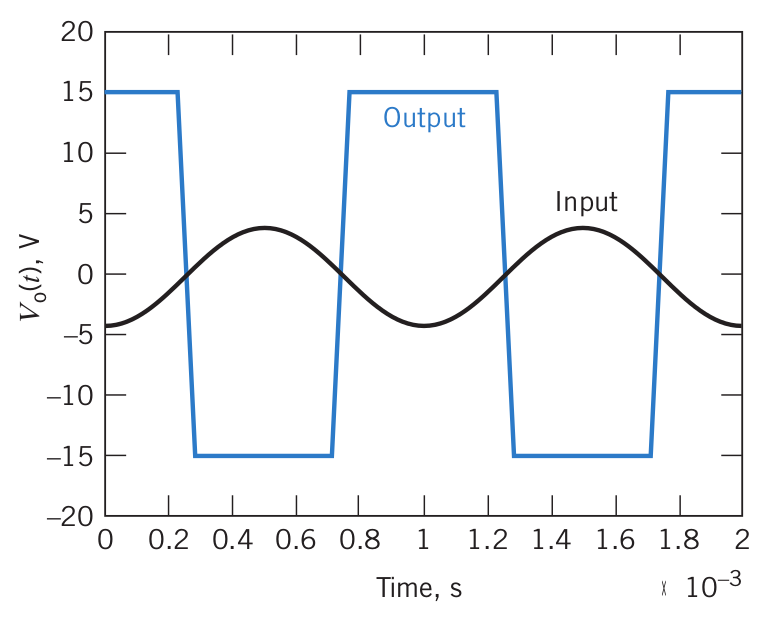
\includegraphics[height=.55\textwidth]{figura29.png}	
		\end{center}
	      \end{column}	
		
	\end{columns}\\
	 \begin{columns}
		\begin{column}{1\textwidth}
		\newline \scalebox{0.8}{\textbf{The correspondence graphic:} $R_{1}=2K\Omega, R_{2}=50K\Omega, v_{s}=-4\cos(2000 \pi t) \ and \ v_{s}=15V$.}
		\end{column}
	\end{columns}\\

\end{tabular}
\end{frame}

\end{document} 